% !TEX root = ../../I4PRJ, Grp3 - Rapport.tex
\chapter{Specifikation og Analyse}
Afsnittet beskriver specifikations- og analysearbejdet. Specifikationsarbejdet begyndte med analyse af projektformulering. Analysen bestod af at løse de problemstillinger som projektformuleringen rejser vha. user stories. Resultatet af analyse arbejdes ses i det tidligere afsnit \todo{ref?? Krav..}. Gruppen bestemte at have fokus på at lave de dele som har mest værdig for slutbrugeren af systemet. User stories blev prioriteret ved en MoSCoW analyse \todo{Reference til metode MoSCow}. Resultatet af kan ligeledes forefindes i \todo{Kravafsnit ref.} i kolonnen MoSCoW. Til at danne overblik over systemets domæner, foretog gruppen en domæneanalyse\todo{ref til metoden domæneanalyse} af user stories. Resultatet af analysen ses i \todo{ref figur med domænemodel}

\begin{figure}
	\centering
	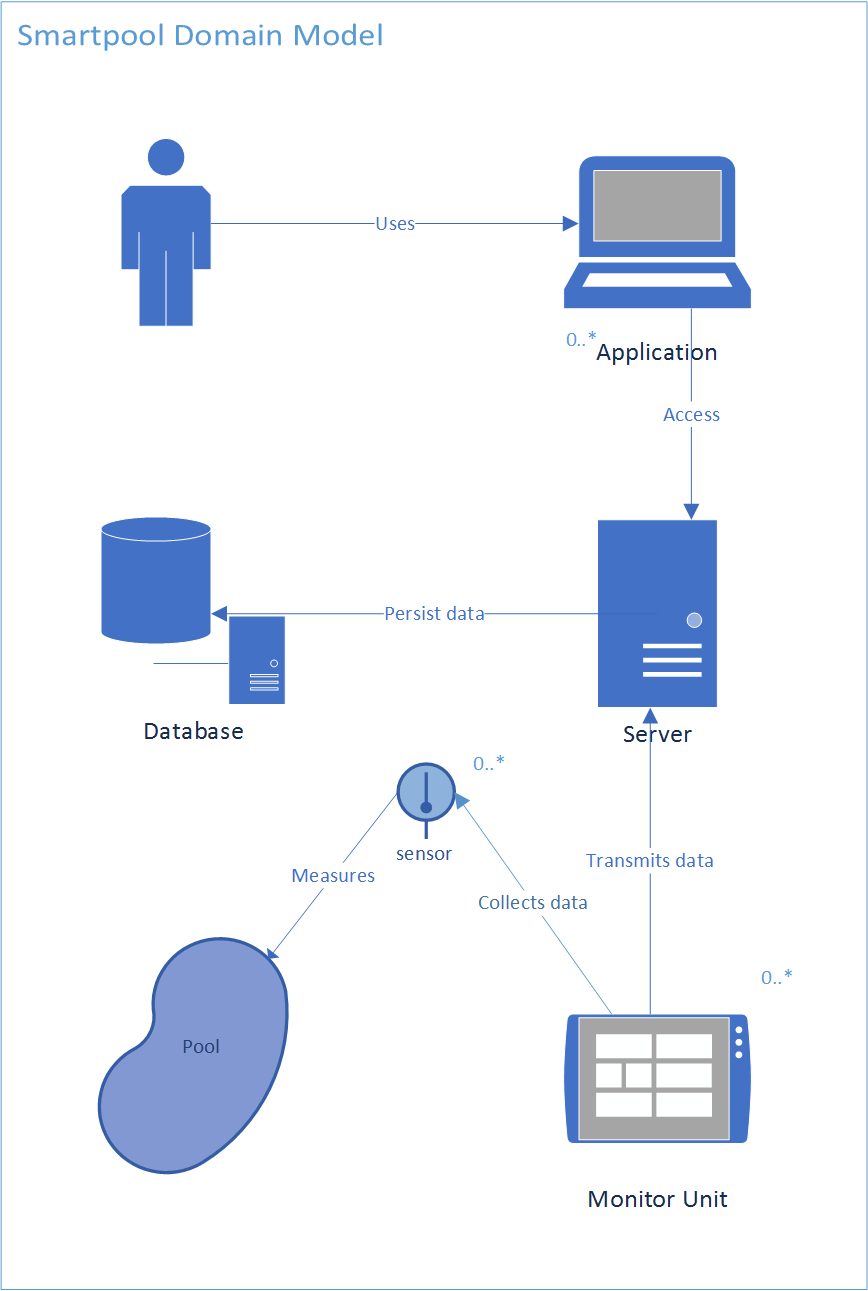
\includegraphics[width=0.8\linewidth]{figs/DomainModelGraphic}
	\caption{Domænemodel for systemet}
	\label{fig:domainmodel}
\end{figure}

{Fig~\ref{fig:domainmodel}

\todo{Indsæt referencen "for domænebeskrivelser se dokumentation}

Smartpool projektet afgrænses til at være foruden dataopsamlingsdelen. \todo{Figuren nedenfor illustrerer projektets afgrænsning}

\begin{figure}
	\centering
	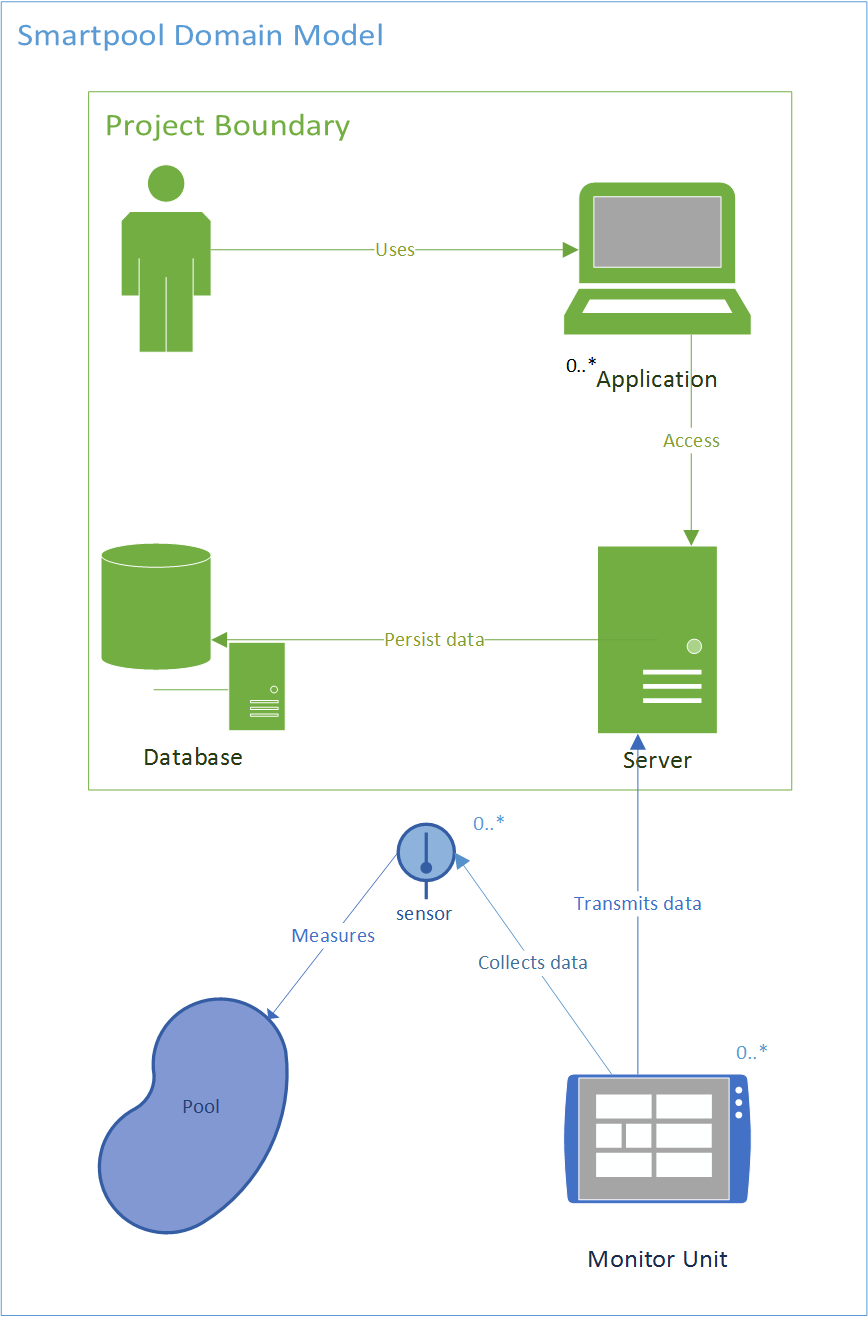
\includegraphics[width=0.8\linewidth]{figs/ProjectBoundary}
	\caption{Domænemodel for systemet}
	\label{fig:domainmodel}
\end{figure}